% !TEX program = xelatex
% !TEX options = -shell-escape -synctex=1 -interaction=nonstopmode -file-line-error "%DOC%"
\documentclass{ctexart}
\usepackage[a4paper,top=1.5cm,bottom=1.5cm,left=2cm,right=2cm,marginparwidth=1.75cm]{geometry}
\usepackage{amsmath}
\usepackage{booktabs}
\usepackage{caption}
\usepackage[colorlinks=false, allcolors=blue]{hyperref}
\usepackage{outlines}
\usepackage{os-common}
\renewcommand{\tableautorefname}{表}

\graphicspath{ {./images/} }

\title{OS笔记}
\author{卢雨轩 19071125}
% \date{\today}
\ctexset{
    section = {
        titleformat = \raggedright,
        name = {,},
        number = 第\chinese{section}部分
    },
    paragraph = {
        runin = false
    },
    today = small,
    figurename = 图,
    contentsname = 目录,
    tablename = 表,
}

\begin{document}

\maketitle
\tableofcontents

\section{操作系统简介}

\subsection{什么是操作系统}

\begin{description}
    \item[系统观点] 操作系统作为资源管理器。记录、协调各个程序对资源的请求。
    \begin{outline}
        \1 硬件资源: 处理器资源、内存、IO设备\dots
        \1 信息资源: 文件管理、锁\dots
    \end{outline} 
    \item[用户观点] 作为机器的拓展。
\end{description}
\subsection{操作系统的历史}
\begin{outline}
    \1 无操作系统
    \1 单道批处理系统
    \1 多道批处理系统
    \1 分时系统、抢占式调度
    \1 现代操作系统
\end{outline}

\subsection{操作系统的基本特征}
\begin{outline}
    \1 并发 Concurrence
    \1 共享 Sharing
    \1 虚拟 Virtual
    \1 异步性 Asynchronism
\end{outline}

\subsection{操作系统的结构}
\begin{outline}
    \1 \emph{整体式结构} 如MS-DOS,Unix。是一系列过程的集合,可以互相调用。
    \1 \emph{层次式结构} 层次式系统的各种功能可以划分为几个层次,每个层次建立在下面的层次之上。 \\
    优点: 模块化 \\
    缺点: 对层的定义;相对效率差 \\
    例子: OS/2
    \1 \emph{微内核结构} 把部分属于操作系统的功能放到内核的外面,使内核更小,称为微内核。
        \2 操作系统微内核之外的进程都是服务进程
        \2 用户进程是客户进程
        \2 微内核中只提供进程管理、内存管理和通讯功能
        \2 系统效率较低(信息传递性能损耗)
    优点:
        \2 易于维护
        \2 易于扩充

\end{outline}
\subsection{操作系统的运行环境}
\subsubsection{程序状态字}
程序状态字(Program State Word, PSW)处于CPU,用于包含状态信息。
\begin{outline}
    \1 Flags(OF,CR,ZERO,\dots)
    \1 \emph{指令优先级}
    \1 \emph{模式(用户、内核)}
    \1 其他控制位
\end{outline}
\subsubsection{双重模式}
\begin{outline}
    \1 监督程序模式(Monitor mode, M Mode):执行OS任务
        \2 Kernel / System / Privileged/ Supervisor mode
        \2 内核模式、系统模式、特权模式、管态
    \1 用户模式(User mode, U mode):执行用户程序
        \2 目态
    \1 区分两种模式的原因:
        \2 提供保护操作系统和其他用户程序的首段
        \2 特权指令:可以引起损害的指令
\end{outline}
\subsubsection{中断}
\begin{outline}
    \1 \emph{现代操作系统是中断驱动的}
    \1 定义:由外部事件引起的暂停过程。
    \1 中断与陷阱:
        \2 中断(Interrupt)指硬中断,如外设、事件
        \2 陷入(Trap)指软中断
\end{outline}

\section{进程管理}
\subsection{进程的概念}
\subsubsection{什么是进程}
进程(Process)是一个正在执行的程序,除了程序代码段等之外包括堆栈段。 

\emph{可重入}指能被多个程序同时调用的程序。纯代码,执行过程中不会改变。
\subsubsection{进程的状态及其转换}

\begin{itemize}
    \item \emph{两状态进程模型} \par
    \adjustbox{valign=t}{
        \begin{minipage}{.5\textwidth}
            \begin{outline}
                \1 进程要么正在被处理器执行,要么没有被处理器执行。
                \1 只有两种状态:
                    \2 运行状态
                    \2 非运行状态
                \1 无法区分等待与就绪
            \end{outline}
        \end{minipage}
    }
    \adjustbox{valign=t}{
        \begin{minipage}{.5\textwidth}
            \begin{center}
                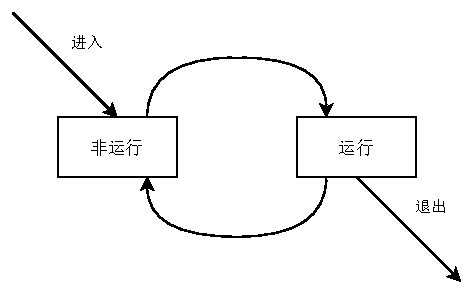
\includegraphics[width=\textwidth]{images/2-state-process-model.pdf}
                \captionof{figure}{两状态进程模型}
            \end{center}
        \end{minipage}
    }

    \item \emph{三状态进程模型} \par
    \adjustbox{valign=t}{
        \begin{minipage}{.5\textwidth}
            \begin{outline}
                \1 三种状态
                    \2 就绪(Ready)
                    \2 运行(Running)
                    \2 等待(Waiting)
            \end{outline}
        \end{minipage}
    }
    \adjustbox{valign=t}{
        \begin{minipage}{.5\textwidth}
            \begin{center}
                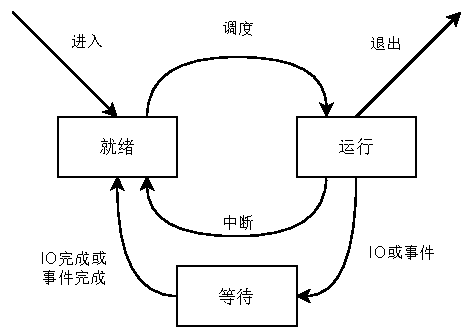
\includegraphics[width=\textwidth]{images/3-state-process-model.pdf}
                \captionof{figure}{三状态进程模型}
            \end{center}
        \end{minipage}
    }
    \item \emph{五状态进程模型} \par
    \adjustbox{valign=t}{
        \begin{minipage}{.5\textwidth}
            \begin{outline}
                \1 五种状态
                    \2 新(New): 进程正在被创建
                    \2 就绪(Ready)
                    \2 运行(Running)
                    \2 等待(Waiting)
                    \2 终止(Stopped):进程已经停止
                \1 缺点:如果所有进程都在等待,CPU利用率低
            \end{outline}
        \end{minipage}
    }
    \adjustbox{valign=t}{
        \begin{minipage}{.5\textwidth}
            \begin{center}
                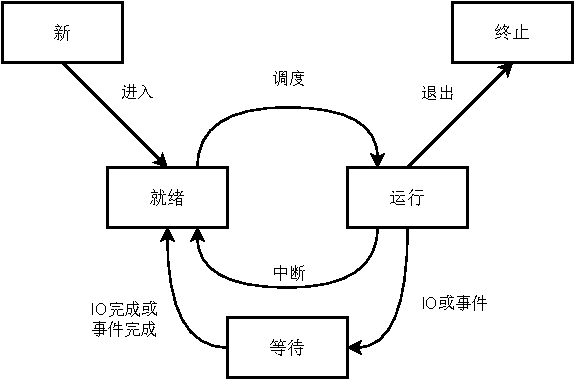
\includegraphics[width=\textwidth]{images/5-state-process-model.pdf}
                \captionof{figure}{五状态进程模型}
            \end{center}
        \end{minipage}
    }
    \item \emph{七状态进程模型} \par
    \adjustbox{valign=t}{
        \begin{minipage}{.5\textwidth}
            \begin{outline}
                \1 七种状态
                    \2 新(New): 进程正在被创建
                    \2 就绪(Ready)
                    \2 运行(Running)
                    \2 等待(Waiting)
                    \2 终止(Stopped):进程已经停止
                    \2 就绪挂起:进程在外存中,等待的事情已经发生
                    \2 等待挂起:进程在外存中,等待的事情还未发生
                \1 提高CPU、内存利用率
                \1 挂起等待中的进程
            \end{outline}
        \end{minipage}
    }
    \adjustbox{valign=t}{
        \begin{minipage}{.5\textwidth}
            \begin{center}
                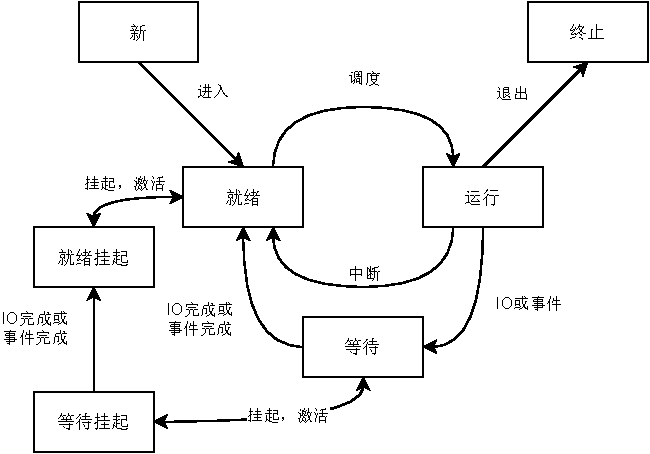
\includegraphics[width=\textwidth]{images/7-state-process-model.pdf}
                \captionof{figure}{七状态进程模型}
            \end{center}
        \end{minipage}
    }
\end{itemize}
\subsubsection{进程的实体与特征}
\begin{outline}
    \1 \emph{进程实体}
        \2 程序代码
        \2 当前的活动
        \2 数据段(data, bss, etc.)
        \2 栈
        \2 堆
    \1 \emph{进程映像}:进程在内存中的组成
        \2 进程控制块(PCB, Process Control Block)
        \2 程序
        \2 数据
        \2 堆栈
    \1 \emph{进程控制块的内容}
        \2 ID
            \3 进程ID
            \3 父进程ID
            \3 用户ID
        \2 当前状态
            \3 寄存器
            \3 栈指针
        \2 常规信息(调度信息,IPC信息,FD,\dots)
\end{outline}
\subsubsection{进程的调度}
\begin{outline}
    \1 \emph{长期调度}
        \2 从进程池中选择进程进入内存
            \3 控制内存中进程的数量
        \2 搭配选择I/O bound和CPU bound程序
        \2 频率低(几分钟一次),有些系统不用
    \1 \emph{中期调度}
        \2 从换出到外存中挂起的进程选择进程进入内存
    \1 \emph{短期调度}
        \2 从就绪队列中选择进程到CPU上执行
        \2 频繁(100ms)
\end{outline}
\subsubsection{进程的特点}
\begin{outline}
    \1 \emph{动态性}:状态在变化
    \1 \emph{并发性}:多个进程可以同时运行
    \1 \emph{独立性}:是独立运行的基本单位
    \1 \emph{异步性}:可以独立的、以不可知的速度运行
\end{outline}

\subsection{
    进程的控制
}
\subsubsection{进程的创建}
\begin{outline}
    \1 进程\emph{通过系统调用}创建进程,前者称为父进程,后者称为子进程
        \2 进程树
    \1 系统调用:
        \2 fork
            \3 共享地址空间,Copy On Write
        \2 execve
            \3 替代地址空间
        \2 spawn
        \2 CreateProcess
\end{outline}
\subsubsection{进程终止}
\begin{outline}
    \1 进程终止自己 exec 系统调用
        \2 父进程使用wait
    \1 父进程终止子进程
        \2 SIGTERM, SIGKILL
        \2 TerminateProcess
    \1 操作系统终止进程
\end{outline}
\subsubsection{进程的阻塞与唤醒}
\begin{outline}
    \1 \emph{阻塞操作} 阻塞的系统调用(调用资源)
    \1 \emph{进程唤醒} 等待的事件到来
\end{outline}
\subsection{进程间通信(IPC)}
\begin{outline}
    \1 \emph{管道通讯}
        \2 管道是一个环形缓冲区
        \2 Producer - Consumer Model
    \1 \emph{共享内存}
        \2 最快
        \2 共享一个内存块
    \1 \emph{消息传递}
        \2 直接通讯:给指定进程发送消息
        \2 间接通讯:『邮箱』
    \1 \emph{同步性问题}: 同步、异步
\end{outline}
\subsection{线程}
\begin{outline}
    \1 \emph{什么是线程}
        \2 \emph{线程}是调度的单位
        \2 \emph{进程}是资源的拥有者
        \2 \emph{轻量级线程},是进程内部的一条运行线
        \2 共享地址空间,拥有线程ID、PC、寄存器和堆栈
    \1 \emph{线程的优点}
        \2 响应度高:不会阻塞整个进程
        \2 资源共享
        \2 通信简单
        \2 经济
    \1 \emph{线程的分类}
        \2 用户级线程
        \2 内核级线程
        \2 混和
\end{outline}
\subsection{进程的同步}
\subsubsection{基础理论}
\begin{outline}
    \1 \emph{进程之间的关系}
        \2 独立的多个进程异步执行,仿佛没有关系
            \3 \sout{独立进程不影响其他进程,也不被其他进程影响?}
            \3 \emph{资源有限!}
        \2 协作的多个进程需要同步
            \3 进程之间可以相互影响
            \3 原因:信息共享;加跨计算;模块化;方便
            \3 例子:Producer-Consumer Model
    \1 \emph{进程同步问题的提出}

    打印机问题。
    
    \1 \emph{竞争条件}

    这种\emph{两个以上的进程共享数据,而最终的执行结果是根据执行次序决定的},
    称为\emph{竞争条件(Data Race)}。

    如何解决Data Race? 控制对资源的访问。

    \1 \emph{临界资源和临界区}

    为了避免竞争条件,必须找到一种方法来阻止多个进程同时读写共享的数据。
        \2 这种共享的数据称为\emph{临界资源 (Critical Resource)}
        \2 程序中访问临界资源的部分称为\emph{临界区 (Critical Section)} 
        \2 \emph{互斥(mutual exclusion)}:
            \3 如果有进程在临界区中执行,那么其他进程都不能在临界区中执行。
            \3 可以避免data race的产生。
        \2 有空让进
        \2 有限等待
        \2 不对进程的相对执行速度进行任何假设

    \1 \emph{如何解决临界区互斥的问题?}
    
        \2 软件的解决方案(Raft等一致性算法?)
        \2 硬件的解决方案
        \2 信号量的解决方案
        \2 管程的解决方案
\end{outline}

\subsubsection{硬件方法}
\begin{outline}
    \1 \emph{硬件的解决方案之一:关中断}

    \emph{进入临界区之前关中断,离开之后开中断}
        \2 线代操作系统是中断驱动的,没有了中断操作系统就失去了控制系统的能力
        \2 只有一个CPU时有效

    \1 \emph{硬件的解决方案之二:原子指令}

    \emph{系统提供了特殊的硬件指令,原子的检查和修改字的内容或者交换两个字。 }
        \2 TestAndSet \\ IBM370 中称为TS指令
        \2 Swap \\ 在 Intel8086 中称为XCHG指令
    
    \1 \emph{TestAndSet}

    \begin{minted}[linenos]{cpp}
bool TestAndSet(bool *target){
    bool value = *target;
    *target = True;
    return value;
}
.....
bool lock;
do {
    // Try to acquire the lock.
    // If can't, busy spin.
    while(TestAndSet(&lock));
    // Lock acquired.
    // Do CRITICAL STUFF.
    lock = False;
    // Release lock for other process.
    // Do REMAINING STUFF.
}
    \end{minted}

    \1 \emph{Swap}
    \begin{minted}[linenos]{cpp}
void Swap(bool *a, bool *b){
    bool value = *a;
    *a = *b;
    *b = value;
}
.....
bool lock;
do {
    bool key = True;
    // Try to acquire the lock.
    // If can't, busy spin.
    while(Swap(&lock, &key));
    // Lock acquired.
    // Do CRITICAL STUFF.
    lock = False;
    // Release lock for other process.
    // Do REMAINING STUFF.
}
    \end{minted}
    \1 \emph{互斥锁(Mutex Locks)}
        \2 底层用TestAndSet或者Swap实现
        \2 acquire()
        \2 release()
    \1 软件和硬件解决方案的问题:
        \2 忙等待(busy waiting)浪费CPU
            \3 解决方案:让出CPU
        \2 优先级反转
            \3 解决方案:优先级捐献
    \1 信号量方法
        \2 两个或多个进程可以用信号进行协作
        \2 进程可以在任何地方停下来等信号
        \2 信号通过Semaphore特殊变量传递信号
        \2 Semaphore操作:
            \3 有一个整形
            \3 wait(P)用来接受信号
            \3 signal(V)用来发送信号
            \3 初值设置为资源数量
        \2 错误使用:
            \3 死锁
            \3 饥饿
    \1 生产者消费者问题
        \2 生产者将任务放入缓冲区
        \2 消费者从缓冲区取出任务
        \2 缓冲区要互斥
            \3 否则会出错
        \2 生产者消费者问题的解决
        \begin{minted}[linenos]{cpp}
semaphore n=0; // 防止consumer消费空队列
semaphore s=1; // 保证put和take操作原子性
semaphore e=N; // 防止producer写入满队列
void producer(){
    while(true){
        a=produce();
        wait(e); // 等待“队列中剩余空位数量”
        wait(s); // 获取队列锁
        put(a);
        signal(s); // 释放队列锁
        signal(n); // 增加“等待处理的任务数量”
    }
}
void consumer(){
    while(true){
        wait(n); // 等待“等待处理的任务数量”
        wait(s); // 获取队列锁
        a=take();
        signal(s); // 释放队列锁
        signal(e); // 增加“队列中剩余空位数量”
        consume(a);
    }
}
        \end{minted}
    \1 哲学家进餐问题
        \2 5个哲学家住在一起,每个人的生活由\emph{吃饭}和\emph{思考}组成
        \2 桌子上有一盘菜,每人一个盘子一支叉子
        \2 想吃饭的哲学家会走到桌子变的位置,拿起左右的叉子,从中间的盘子中去菜放到自己的盘子中
        \2 要求:
            \3 保证叉子互斥
            \3 防止死锁和饥饿
    \1 读者写者问题
        \2 可以同时读,有人写别人就不能读/写
        \2 读者优先:
        \begin{minted}[linenos]{cpp}
int readcount=0;
semaphore x=1; // 保证readcount操作原子性
semaphore wsem=1;
void reader()
{
    while(1){
        wait(x);
        readcount++;
        if(readcount==1)
            wait(wsem); // 第一个读者锁住锁
        signal(x);

        READUNIT();

        wait(x);
        readcount--;
        if(readcount==0)
            signal(wsem);
        signal(x);
    }
}
void writer()
{
    while(1)
    {
    wait(wsem);
    WRITEUNIT();
    signal(wsem);
    }
}
        \end{minted}
        \2 写者优先:
        \begin{minted}[linenos]{cpp}
int readcount=0, writecount=0;
semaphore x=1, y=1, z=1, wsem=1, rsem=1;
void reader()
{
    while(1){
        wait(z);
        wait(rsem);
        wait(x);
        readcount++;
        if(readcount==1)
            wait(wsem);
        signal(x);
        signal(rsem);
        signal(z);
        READUNIT();
        wait(x);
        readcount--;
        if(readcount==0)
            signal(wsem);
        signal(x);
    }
}
void writer()
{
    while(1){
        wait(y);
        writecount++;
        if(writecount==1)
            wait(rsem);
        signal(y);
        wait(wsem);
        WRITEUNIT();
        signal(wsem);
        wait(y);
        writecount--;
        if(writecount==0)
            signal(rsem);
        signal(y);
    }
}
    \1 信号量的问题:
        \2 操作系统提供
        \2 有效,灵活
        \2 容易死锁
    \1 管程
        \2 管程用条件变量的方法支持同步。
        \2 条件变量在管程内部,只能由管程访问。
        \2 在条件变量C上可以有两种操作:
        \end{minted}
\end{outline}
\subsubsection{死锁}
\begin{outline}
    \1 死锁的定义
        \2  如果一个进程集合中每一个进程都在等待只能由 本集合中的另一个进程才能引发的事件,则称这 种状态为死锁。
    \1 死锁的条件
        \2 互斥
            \3 一个资源同时只让一个进程使用
        \2拥有并等待
            \3 进程在拥有一个资源时又申请另一个资源,并等待分配给它。
        \2 资源不可抢占
            \3 分配给一个进程的资源是不可抢占的,只能由占有它的进程释放
        \2 环路等待
            \3 进程和资源之间存在一个拥有和需求的闭环
    \1 资源分配图:
        \2 有环就可能有死锁
        \2 需要每个资源有一个实例
    \1 死锁的解决
        \2 忽略
        \2 预防死锁
        \2 避免死锁
        \2 死锁的检测和恢复
\end{outline}


\end{document}
